% Metódy inžinierskej práce

\documentclass[10pt,twoside,slovak,a4paper]{article}

\usepackage[slovak]{babel}
\usepackage[T1]{fontenc}
\usepackage[IL2]{fontenc} % lepšia sadzba písmena Ľ než v T1
\usepackage[utf8]{inputenc}
\usepackage{graphicx}
\usepackage{url} % príkaz \url na formátovanie URL
\usepackage{hyperref} % odkazy v texte budú aktívne (pri niektorých triedach dokumentov spôsobuje posun textu)

\usepackage{cite}
%\usepackage{times}

\pagestyle{headings}

\title{Evolúcia počítaťových hier\thanks{Semestrálny projekt v predmete Metódy inžinierskej práce, ak. rok 2022/23, vedenie: Ing. Ivan Kapustík}} % meno a priezvisko vyučujúceho na cvičeniach

\author{Dávid Babiš\\[2pt]
	{\small Slovenská technická univerzita v Bratislave}\\
	{\small Fakulta informatiky a informačných technológií}\\
	{\small \texttt{xbabis@stuba.sk}}
	}
	

\date{\small 17.10.2022} % upravte



\begin{document}

\maketitle

\begin{abstract}
To, že sa počítačové hry z roka na rok menia a vylepšujú, nie je pre vás určite novinkou. Vidieť ju však v rozmedzí mnoho rokov je zaručene niečo neopísateľné. Počítačová technika ide neuveriteľne rýchlo dopredu. Tieto hry sú s nami iba pár desiatok rokov, ale za tú dobu sa stihli výrazne zmeniť. Od jednoduchých pixelov na čiernobielych monitoroch sme sa dostali k prepracovanej grafike, ktorá nielen verne zachytáva našu skutočnosť, ale dokáže vykresliť aj neskutočnosť. Napríklad fantastické svety ktoré existujú len vo videohrách.  V tomto článku sa dozviete, ako sa menila nielen grafická stránka počítačových hier od roku 1952. Rozdiel je naozaj obrovský. Pamätáte si ešte niektoré staré klasiky?
\end{abstract}



\section{Úvod}
Ak sa chcete dozvedieť viac o vývine počítačových hier, zdokonaliť sa alebo ste o pc hrách ešte nič nevedeli, ste tu na správnom mieste. V tomto článku sa spoločne pozrieme na počítačové hry, ich históriu a rozdelenie podľa žánrov. Tiež si porovnáme starú a novú verziu jednej kultovej hry, a ukážeme si ako sa časom z hľadiska mechaniky a grafiky zmenila. Ešte sa pozrieme na evolúciu počítačových hier všeobecne, v priebehu desiatok rokov. V závere si tento pokrok ešte zhrnieme. História pc hier naznačená v úvode, je podrobnejšie vysvetlená v časti~\ref{historia}. Porovnanie zmien v konkrétnej videohre nájdete v časti~\ref{porovnanie}. 
Dôležité súvislosti s rozdelením videohier podľa žánrov sú uvedené v časti~\ref{zanre}.
Záverečné poznámky prináša časť~\ref{zaver}.

\section{História počítačových hier} \label{historia}

\subsection{NIMROD 1951}

V roku 1951 bol pri príležitosti "Festival of Britain" predstavený digitálny počítač Ferranti NIMROD. Išlo o prvý počítač navrhnutý špeciálne pre počítačovú hru. Tento stroj so spotrebou krásnych 6 kilowattov a frekvenciou procesora 10kHz vedel, ako už názov napovedá, jedinú hru - NIM. Pôvodom pravdepodobne v Číne, NIM je jednoduchá logická hra pre dvoch hráčov spočívajúca v odoberaní prvkov z niekoľkých (typicky troch) množín. V každom ťahu môže hráč odobrať ľubovoľné množstvo prvkov (miniálne jeden) z jednej množiny. Víťazom je ten hráč, ktorý odoberie posledný prvok.

Ako „grafický“ výstup bol použitý panel so žiarovkami. NIMROD teda nie je mnohými považovaný za skutočnú videohru, pretože nepoužíva zobrazovacie zariadenie typu TV/monitor a pod. Ale to sa zase dostávame k problematickej definícii videohry. O niečo neskôr bol NIMROD s veľkým úspechom vystavený aj v Berlíne.



\subsection{OXO 1952} \label{nejaka}

Za prvú skutočnú videohru je možné OXO považovať najmä preto, že pre jej grafický výstup bola vôbec prvýkrát v dejinách počítačov použitá osciloskopická obrazovka, teda monitor.Vznikla v roku 1952.  Zobrazenie bitmapy bolo 35 × 16 pixelov. Hra bola nainštalovaná na elektrónkovom počítači EDSAC, ktorý bežne používal dierne pásky. Zahrať ste si mohli jedine proti umelej inteligencii. Ovládať ju bolo možné pomocou vytáčacieho telefónu, pričom vytočené číslo znamenalo políčko, na ktoré hráč umiestnil guľôčku alebo krížik.
Hra bola na počítači EDSAC nainštalovaná iba po dobu Douglesovej dizertačnej práce a širokej verejnosti sprístupnená nikdy nebola. Po obhájení svojej práce musel Douglles hru z počítača vymazať, pretože zaberala príliš mnoho miesta. 

Z obr.~\ref{f:rozhod} je všetko jasné. 

\begin{figure*}[tbh]
\centering
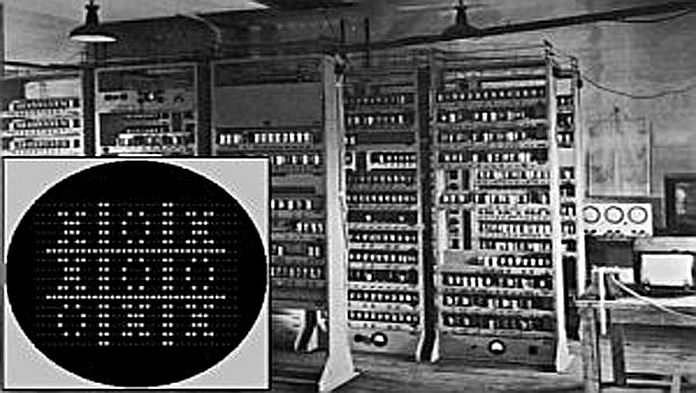
\includegraphics[scale=0.5]{Schránka-15.jpg}
%Aj text môže byť prezentovaný ako obrázok. Stane sa z neho označný plávajúci objekt. Po vytvorení diagramu zrušte znak \texttt{\%} pred príkazom \verb|\includegraphics| označte tento riadok ako komentár (tiež pomocou znaku \texttt{\%}).
\caption{Rozhodujúci argument.}
\label{f:rozhod}
\end{figure*}



\section{Žánre počítačových hier} \label{zanre}

Základným problémom je že hry majú mnoho podôb a niekedy je ťažké ich rozlíšiť. Preto má vačšina hier priradených viac žánrov zároveň. Niektoré využívajú PvP\footnote{Player versus player - hráč proti hráčovi.}, iné zase AI\footnote{Artificial intelligence - umelá inteligencia.}.

Najprv sa pozrieme na nejaké vysvetlenie (časť~\ref{zanre:adventure}), a potom na ešte nejaké (časť~\ref{zanre:akcne}).

Môže sa zdať, že problém vlastne nejestvuje\cite{Coplien:MPD}, ale bolo dokázané, že to tak nie je~\cite{Czarnecki:Staged, Czarnecki:Progress}. Napriek tomu, aj dnes na webe narazíme na všelijaké pochybné názory\cite{PLP-Framework}. Dôležité veci možno \emph{zdôrazniť kurzívou}.


\subsection{Akčné hry} \label{zanre:akcne}

Patria sem rôzne bojové hry ale aj strielačky. Dôležitou vlastnosťou je mať dobré reflexy pretože hra sa odohráva v reálnom čase a hráč je pod nátlakom a má málo času na rozhodovanie. Hráči majú k dispozícii rôzne strelné a tiež ručné zbrane, granáty, nožíky a podobne. Akčné hry sú väčšinou časovo obmedzené. Tento žáner zvyčajne spojený s jedným z ostatných žánrov. Napríklad akčné adventúry alebo akčné RPG. Žánre ktoré vychádzajú z akčných hier sú napríklad FPS alebo Battle Royale.


\subsection{Dobrodružné hry} \label{zanre:adventure}

Najskôr mali textovú podobu, no postupne sa vyvíjali až do dnešnej podoby, kde už ide o rozsiahle konverzácie postáv, rôzne zápletky, hádanky a bohatý príbeh. Ide väčšinou o single player hry, ale existujú aj takzvané co-op\footnote{Kooperatívne hry - skupina ľudí hrá hru, v ktorej hrajú na rovnakej strane, napríklad proti počítaču.}hry. Adventúry majú zvyčajne jednu hlavnú dejovú líniu a veľa vedlajších, tzv. side questov. Vyskytujú sa v nich aj rôzne easter eggy\footnote{Easter egg alebo veľkonočné vajíčko je skrytá a oficiálne nedokumentovaná funkcia alebo vlastnosť počítačového programu. Veľkonočnými vajíčkami môžu byť neškodné minihry, vtipné funkcie, neobvyklé, implicitne nedefinované správanie programu, rôzne animácie, grafické symboly, titulky s menami tímu programových tvorcov.}. Hráč sa posúva v príbehu ďalej interakciou s prostredém, komunikáciou s rôznymi postavami, riešením hádaniek, zbieraním a používaním rôznych predmetov. Väčšinou ide o hry kde sa preskúmavajú hrobky, stratené mestá, hľadá sa poklad a podobne. Hráč sa môže nachádzať aj vo fiktívnom svete plného magických postáv, zvierat a predmetov. ale existujú aj realistické adventúrne hry. Adventúry nemajú na vyhranie kampane žiadny časpvý limit.

Príklady dobrodružných hier:
\begin{itemize}
\item Séria videohier Uncharted
\item Séria videohier Tomb Raider
\item The Last of Us
\item Days Gone
\item Death Stranding
\item Horizon Zero Dawn
\end{itemize}

\begin{figure*}[tbh]
\centering
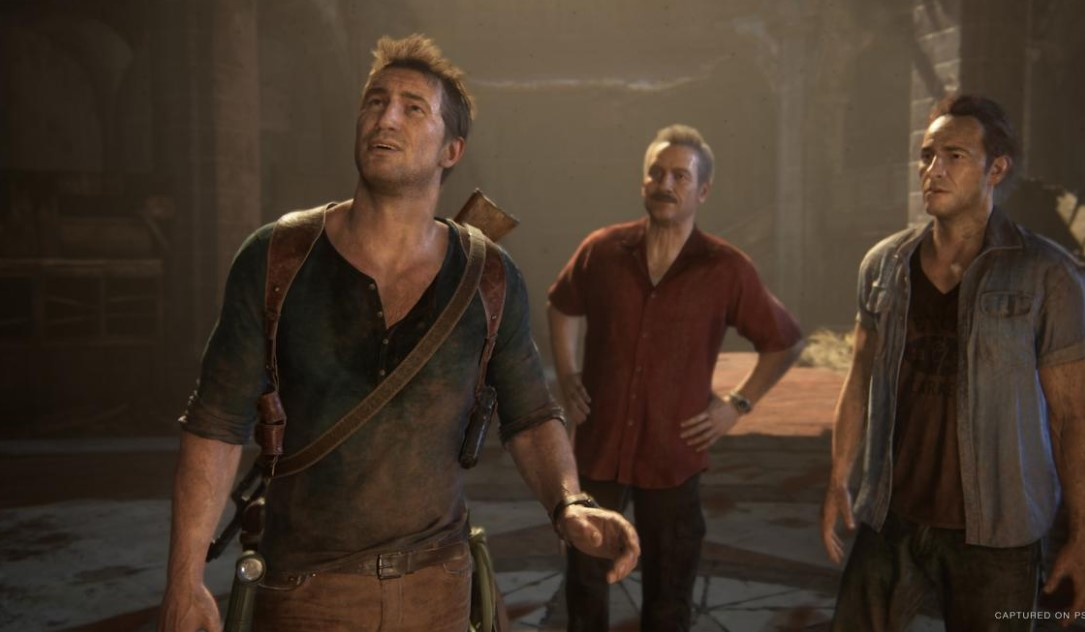
\includegraphics[scale=0.3]{Screenshot.jpg}
\caption{Screenshot z dobrodružnej hry Uncharted 4}
\label{f:uncharted}
\end{figure*}


\subsection{FPS} \label{zanre:fps}

First person shooter alebo strielačka z prvého pohľadu je asi najzámejší žáner videohier. Mnohé klasiky sú v tomto 

Príklady FPS hier:
\begin{itemize}
\item Counter-Strike: Global Offensive
\item Counter-Strike 1.6
\item Rainbow Six: Siege
\item Séria videohier Call of Duty
\item Séria videoheir Battlefield
\item Séria videoheir Halo
\end{itemize}

\begin{figure*}[tbh]
\centering
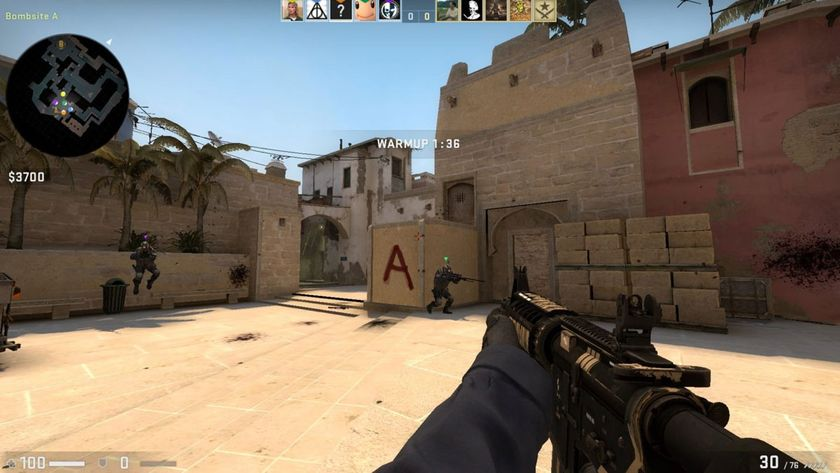
\includegraphics[scale=0.2]{csgo.jpg}
\caption{Screenshot z hry Counter-Strike: Global Offensive}
\label{f:csgo}
\end{figure*}

\subsection{Battle Royale} \label{zanre:battleroyale}

Battle royale hry sú pomerne nový žáner. Sú veľmi podobné akčným hrám, s tým rozdielom že battle royale hry nemajú príbeh a ide hlavne o to, aby si hráč čo najviac užil a vychutnal akciu. Hlavným znakom je že hráči bojujú medzi sebou, každý proti každému. Hra sa odohráva na nejakom ostrove alebo na vymedzenej časti pevniny. Nachádza sa tu bezpečná zóna, ktorá je najskôr na celej mape, ale tá sa postupne zmenšuje a to núti hráčov k častejšiemu stretávaniu a konfliktom. Bezpečná zóna sa zmenšuje dovtedy, kým sú nažive ešte aspoň dvaja hráči. Ak hráč vystúpi z bezpečnej zóny postupne stráca životy a zomiera. Všetci hráči majú dostupnú mapu ostrova s vyznačenými lokalitami a bezpečnou zónou, prázdny inventár. Každý hráč má na začiatku hry rovanký počet životov a žiadne zbrane. Hra je väčšinou až pre 100 hráčov. Hráči začínajú hru niekde mimo ostrova, a po pripojení všetkých 100 hráčov, sa hráči presunú do lietadla, ktoré letí ponad mapou. Sami sa môžu rozdodnúť kde a kedy vyskočia z lietadla, a pomocou padáku pristanú na ľubovolnom mieste na mape. Po celej mape sú náhodne rozmiestnené zbrane a vozidlá. Cieľom hry je zbierať a vylepšovať rôzne zbrane a zvyšovače životov, liečiť sa, bojovať s ostatnými hráčmi, postupne sa presúvať po mape kvôli zmenšovaní bezpečnej zóny, prežiť a vyhrať. Hru vyhráva posledný živý hráč. Hra trvá približne 20-30 minút. Ide vždy o online hry.

Príklady Battle royale hier:
\begin{itemize}
\item Fortnite
\item PlayerUnknown's Battlegrounds
\item Apex Legends
\item Call of Duty: Warzone
\item H1Z1
\item Battlefield V
\end{itemize}

\begin{figure*}[tbh]
\centering
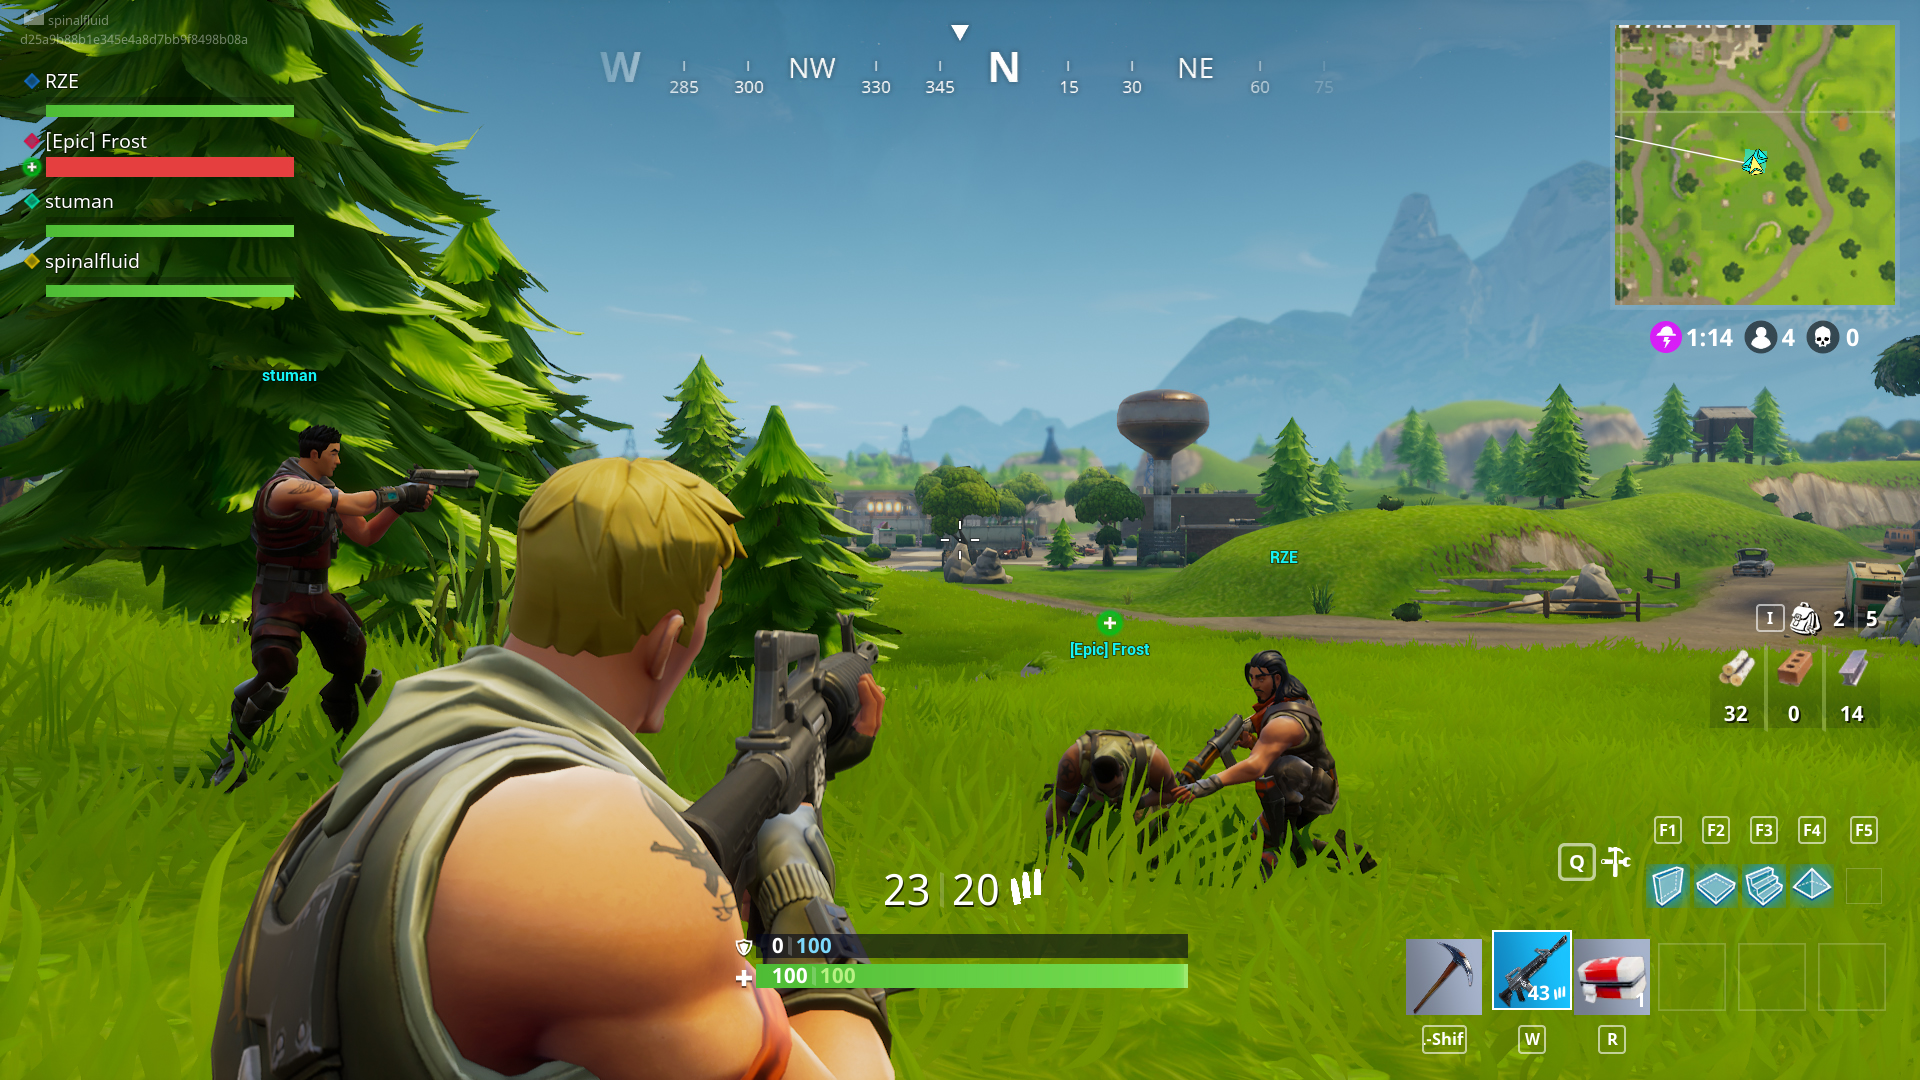
\includegraphics[scale=0.15]{fortnite.jpg}
\caption{Screenshot z hry Fortnite}
\label{f:fortnite}
\end{figure*}

\subsection{Sandbox} \label{zanre:sanbox}

Hlavným znakom tohto žánru je otvorený svet, ktorý ponúka svojim hráčom obrovské možnosti na úpravu a tvorbu prostredia. Cieľ si sám kladie hráč, ktorý sa môže slobodne rozhodovať čo spraví ďalej. Tento žáner podporuje u hráča tvorivosť. 

Príklady Sandbox hier:
\begin{itemize}
\item Minecraft
\item Séria videohier Grand Theft Auto
\item Raft
\item Watch Dogs
\item Just Cause 4
\item No Man's Sky
\end{itemize}

\begin{figure*}[tbh]
\centering
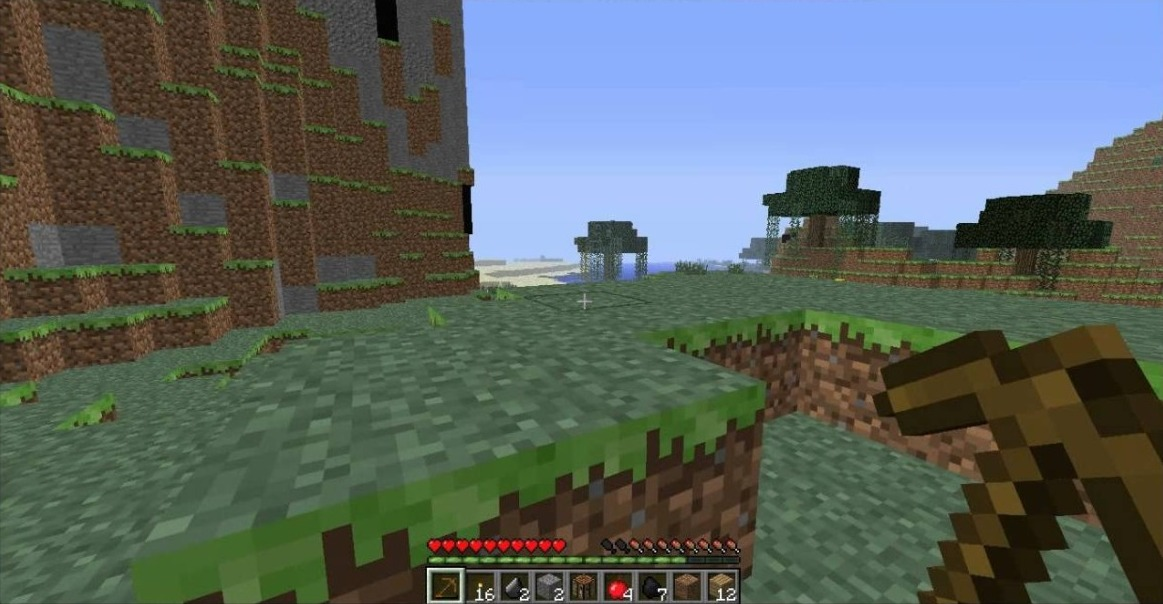
\includegraphics[scale=0.15]{minecraft.jpg}
\caption{Screenshot z hry Minecraft}
\label{f:minecraft}
\end{figure*}

\subsection{Strategické hry} \label{zanre:strategicke}

Sú určené pre hráčov, ktorých baví rôzne plánovanie útokov, vymýšlanie stratégií a rýchle konanie. Cielom je pomocou svojich bojových zručností, skúseností a dôvtipu vyhrať nad nepriateľom. Hráči svoje ťahy pečlivo plánujú a snažia sa prechytračiť oponenta. Svoju taktiku môžu meniť podľa vývoju hry. Stratégie sú vačšinou zasadené do stredoveku, kde bojujú pomocou vtedajších zbraní. Často má hráč na starosti napríklad nejakú pevnosť alebo kráľovstvo, a jeho úlohou je ju brániť, postupne zlepšovať obranu a hlavne útočiť na pevnosti ostatných hráčov. Tieto hry sú väčinou v online móde, ale môžu mať aj single player.  Typickou strategicou hrou je napríklad šach.

Príklady strategických hier:
\begin{itemize}
\item Clash of Clans
\item Séria videohier Settlers
\item Age of Empires
\item CIVILIZATION VI
\end{itemize}

\begin{figure*}[tbh]
\centering
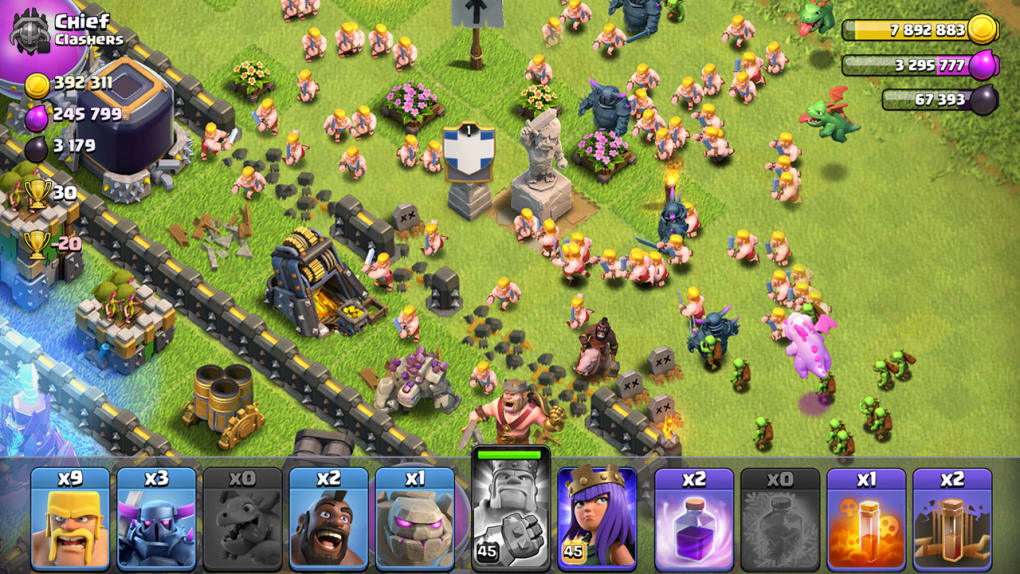
\includegraphics[scale=0.3]{coc.jpg}
\caption{Screenshot z hry Clash of Clans}
\label{f:coc}
\end{figure*}

\subsection{RPG} \label{zanre:rpg}



\subsection{Simulátory} \label{zanre:simulatory}

V týchto hrách ide o simuláciu reálneho života, cielom je hlavne zabaviť sa, a to spôsobom robenia niečoho, čo v realite buď nemôžeme robiť alebo nevieme robiť a chceme sa to naučiť. Existuje mnoho simulátorov, najznámejšie sú Euro Truck Simulator, Farming Simulator, Flight Simulator a veľa ďalších. V skratke, existuje simulátor skoro na čokoľvek čo sa dá vykonávať v reálnom svete. Nejde o to hru vyhrať, a ani sa nedá vyhrať, ale hrať dovtedy, kým to hráča bude baviť.

Príklady simulátorov:
\begin{itemize}
\item Euro Truck Simulator 2
\item Farming Simulator
\item Flight Simulator
\item Séria videohier The Sims
\item Séria videohier Fifa
\item Séria videohier The Show
\end{itemize}

\begin{figure*}[tbh]
\centering
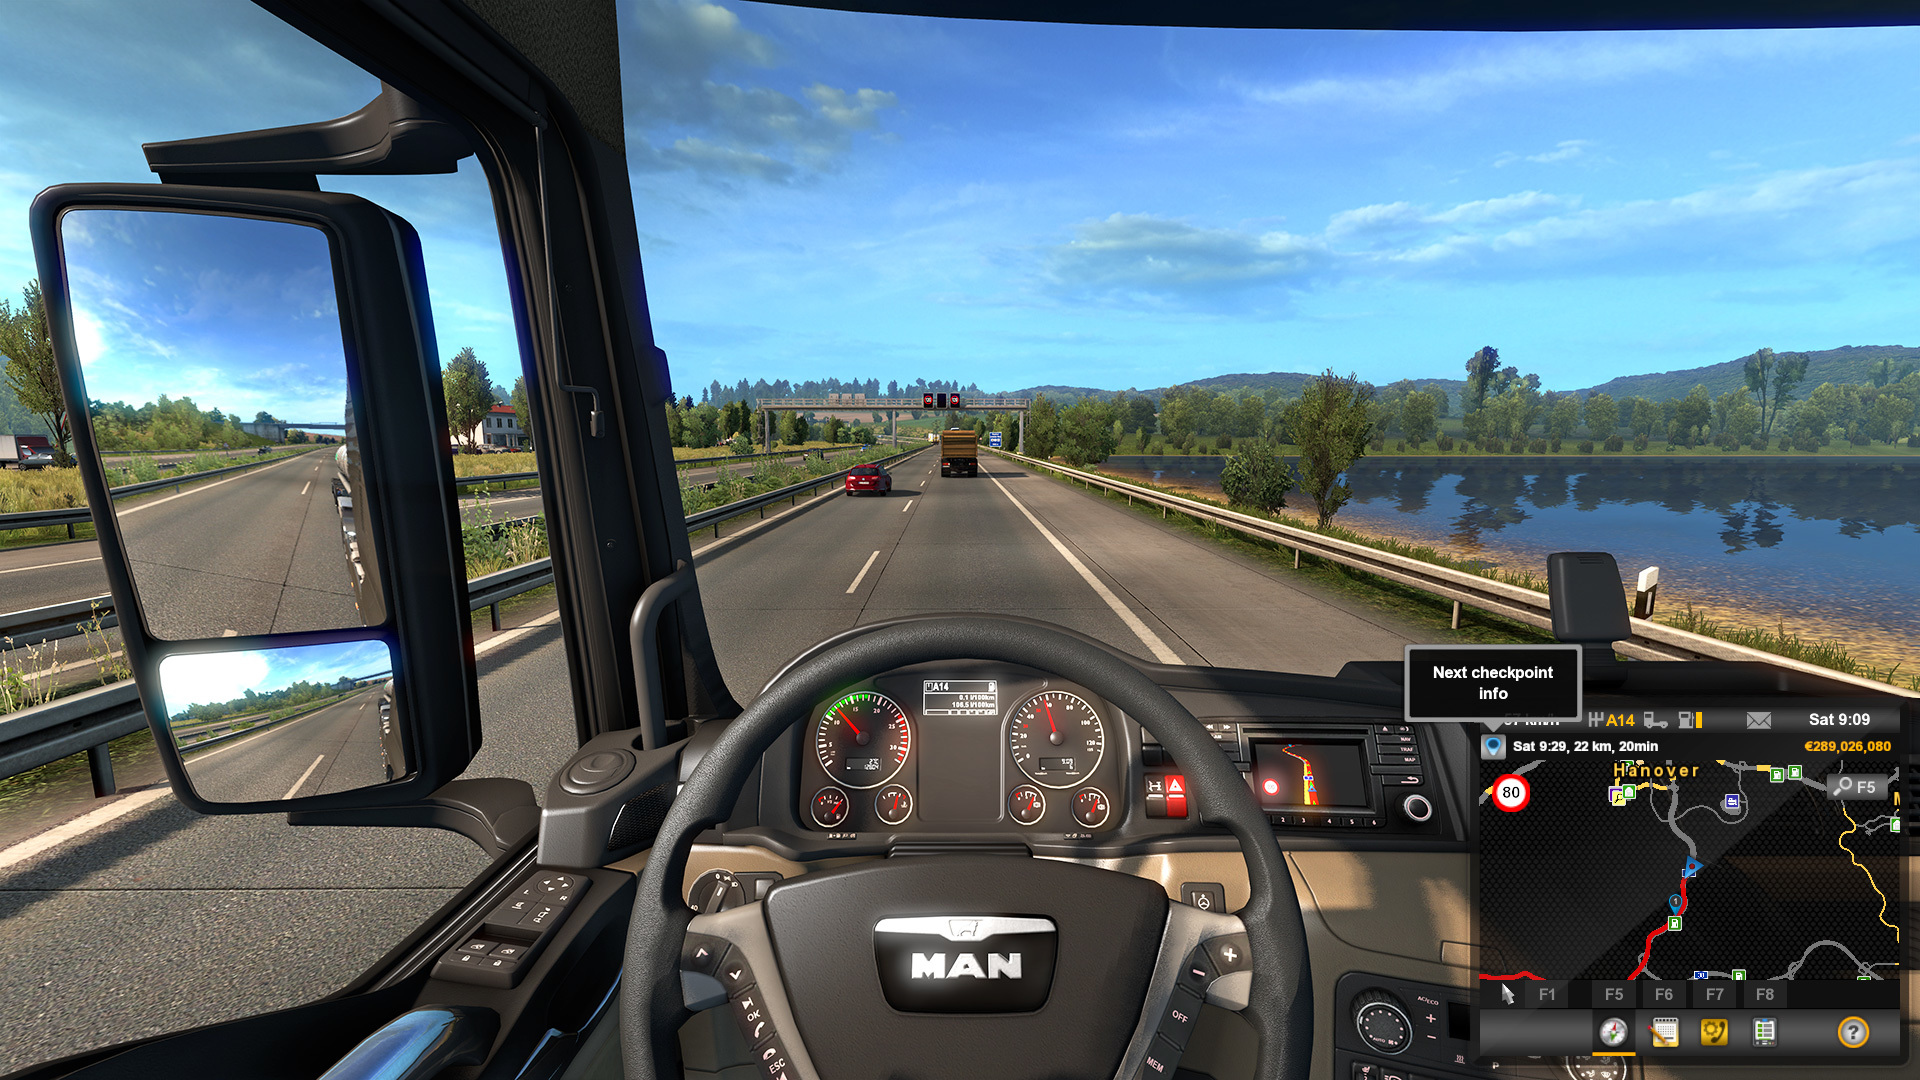
\includegraphics[scale=0.15]{ets.jpg}
\caption{Screenshot z hry Euro Truck Simulator 2}
\label{f:ets2}
\end{figure*}

\section{Porovnanie CS 1.6 a CS:GO} \label{porovnanie}

Akčnú FPS hru Counter-Strike asi netreba nikomu predstavovať. Legendárna hra ktorú si obľúbili milióny hráčov vznikla ako modifikácia obľúbenej hry Half-Life ešte v roku 1999. Od tej doby hra prešla mnohými úpravami. Ako samostatná hra vyšla v roku 2003 s názvom Counter-Strike 1.6 . Poďme sa teda spoločne pozrieť ako sa zmenila nielen po grafickej stránke v priebehu rokov. Budeme porovnávať jej úplne prvú verziu CS 1.6, s tou najnovšou, a to je Counter-Strike: Global Offensive (2012). Tak poďme sa nato pozrieť.

\begin{figure*}[tbh]
\centering

\includegraphics[scale=0.8]{cs16.png}
\caption{CS 1.6 logo}
\label{f:cs1.6}
\end{figure*}

\subsection{Engine} \label{porovnanie:engine}

Enginy a všetky verzie Counter-Strikeu
\begin{enumerate}
\item Engine GoldSrc
	\begin{enumerate}
	\item Couter-Strike Beta 1
	\item Couter-Strike Beta 2
	\item Couter-Strike Beta 3
	\item Couter-Strike Beta 4
	\item Couter-Strike Beta 5
	\item Couter-Strike Beta 6
	\item Couter-Strike Beta 7
	\item Couter-Strike 1.0
	\item Couter-Strike 1.1
	\item Couter-Strike 1.2
	\item Couter-Strike 1.3
	\item Couter-StrikeCS 1.4
	\item Couter-Strike 1.5
	\item Couter-Strike 1.6
	\item Couter-Strike: Condition Zero (CS:CZ)
	\end{enumerate}
\item Engine Source
	\begin{enumerate}
	\item Couter-Strike: Source (CS:S)
	\item Couter-Strike: Global Offensive (CS:GO)
	\end{enumerate}
\end{enumerate}

Zatiaľ čo 1.6 bežala na engine GoldSrc, CS:GO beží na engine Source od Valve Coproration. Source 3D engine bol vytvorený spoločnosťou Valve Software v roku 2004. Primárne bol určený pre hru Half-Life 2. Jeho základom bol predchádzajúci engine GoldSrc, čo bola silne upravená verzia Quake enginu.

\subsection{Grafika} \label{porovnanie:grafika}

Už na prvý pohľad vieme rozlíšiť CS 1.6 a CS:GO. Grafika 1.6 bola na svoju dobu veľmi pokroková. V denšnej dobe je grafika  CS:GO na vysokej úrovni a dokáže konkurovať aj ostatným kvalitným videohrám. Dnešná grafika je už skoro na nerozoznanie od reality, ale je to skutočne pravda? Toto isté si hovorili aj hráči na konci deväťdesiatych rokov keď zbadali CS 1.6 . Uvidíme ako to bude s hernou grafikou v budúcnosti. Pri súčašných technológiách ako je napríklad virtuálna realita je len otázkou času, kedy naozaj nerozoznáme hru od reality. Určite sa máme na čo tešiť.

\begin{figure*}[tbh]
\centering
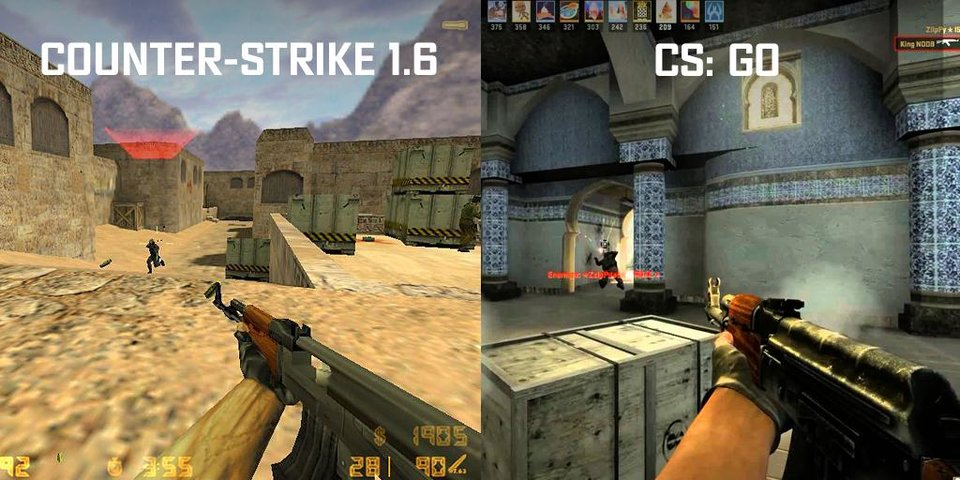
\includegraphics[scale=0.4]{1.6vsgo.jpg}
\caption{Porovnanie grafiky}
\label{f:grafika}
\end{figure*}

\subsection{Skiny} \label{porovnanie:skiny}

Zatiaľ čo CS 1.6 nemala mnoho skinov na zbrane a boli väčšinou iba výsadov niektorých serverov, CS:GO ich má tisíce a stále pribúdajú. Ich hodnota sa vyjadruje v reálnych peniazoch, ale pritom ide o virtuálnu položku v počítači. Ich cena závisí od množstva existijúcich skinov alebo od krásy jednotlivého skinu. Vzácnych skinov je málo a preto sú aj oveľa drahšie. Skiny sa dajú kupvať a predávať anonymne cez virtuálny marketplace Steam market, alebo aj vymienať s ostatnými hráčmi.
Skiny sa dajú zadarmo získať buď z dropov po každej hre, alebo si ich musí hráč kúpiť cez Steam market alebo od iného hráča. Skiny môže hráč ešte získať z debien, na ktorých odomknutie je treba virtuílny kľúč, ktorý ale nieje zadarmo. Hráč si ho musí kúpiť. Otvorenie debny funguje na princípe herných automatov, s tým rozdielom že hráč vždy dostane nejaký skin. Ale nie každý skin je vzácny a tým pádom aj dosť drahý na to aby hráč získal nejaký ten profit z otvorenia debny. Otvorenie jednej debny stojí okolo troch eur. A je veľmi malá šanca aby hráč získal z debny skin ktorý je drahší ako náklady na otvorenie jednej debny, a ešte menšia šanca aby získal niečo veľmi vzácne. Je veľmi ľahké na tom prerobiť, a preto by mal každý hráč zvážiť či mu peniaze stoja za to riziko. Tieto virtuálne kasína sú nebezpečné.

\begin{figure*}[tbh]
\centering
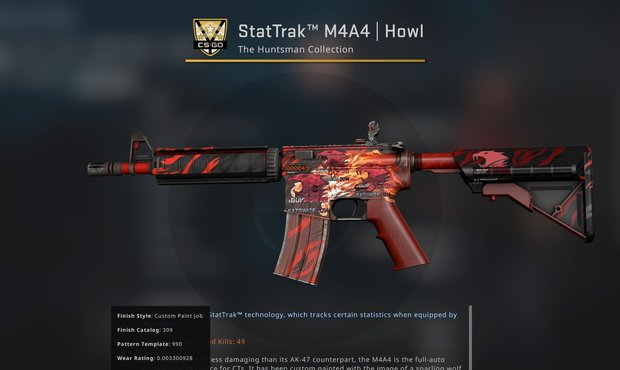
\includegraphics[scale=0.8]{skin.jpg}
\caption{Ukážka jedného skinu na zbraň M4A4}
\label{f:skiny}
\end{figure*}


\section{Evolúcia v priebehu desiatok rokov} \label{evolucia}




\section{Záver} \label{zaver} % prípadne iný variant názvu


%\input{example.tex}



%\acknowledgement{Ak niekomu chcete poďakovať\ldots}


% týmto sa generuje zoznam literatúry z obsahu súboru literatura.bib podľa toho, na čo sa v článku odkazujete
\bibliography{literatura}
\bibliographystyle{alpha} % prípadne alpha, abbrv alebo hociktorý iný
\end{document}
